\FloatBarrier
\section{Empirical Demonstration: Chicago Energy Benchmarking}

Section 3 established the three TDGP stages in the abstract: read the recording layer from the data (Stage 1), hypothesise the world layer (Stage 2), and test that hypothesis against the primary institutional documentation (Stage 3). This section carries all three out on the Chicago Energy Benchmarking data. Subsections 4.2 through 4.4 apply each stage in sequence; Sections 5 to 7 then carry out the analysis the tested DAG licenses.


\subsection{Dataset and Institutional Context}

The dataset is drawn from the City of Chicago Data Portal (\cit{citynd}{City of Chicago, n.d.}) and covers 28,329 building-year records across ten annual reporting cycles (2014--2023), representing 3,852 unique buildings. Coverage grew from 243 records in 2014 to approximately 3,400--3,600 per year from 2018 onward, reflecting the programme's phased expansion and improving compliance rates (Figure 4.1). The 29 variables fall into five natural groups that also mark five positions in the data-generating process. Table 4.1 lists them with their observation rates from our analysis of the dataset.

\begin{figure}[tbp]
\centering
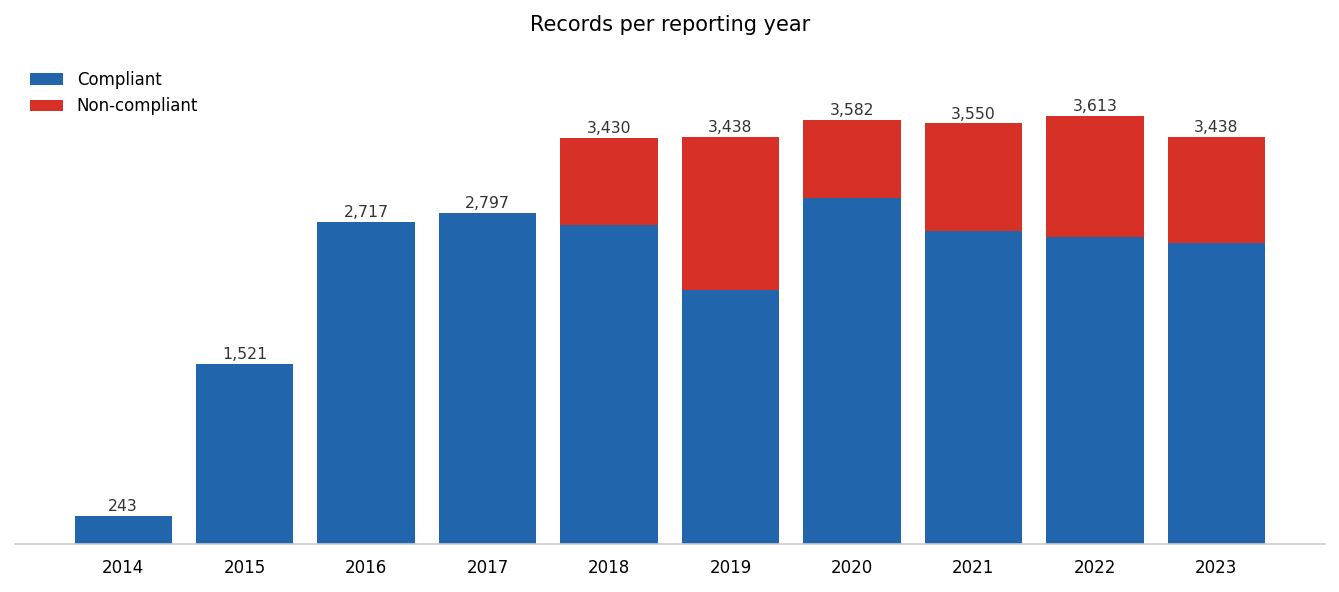
\includegraphics[width=0.85\linewidth]{figures/fig_01_records_per_year.png}
\caption*{\textbf{Figure 4.1. Dataset coverage by reporting year, stacked by compliance status.} Records grew steeply from 2014 to 2018 as the programme was phased in, then stabilised at roughly 3,400--3,600 per year. Compliant records (blue) consistently outnumber non-compliant (red) in every year. Author's analysis of Chicago Energy Benchmarking data (\cit{citynd}{City of Chicago, n.d.}).}
\end{figure}

\par\medskip\noindent
{\small\itshape \textbf{Table 4.1. Variable inventory by SCM role.} Observation counts and null rates are the author's analysis of the Chicago Energy Benchmarking dataset (\cit{citynd}{City of Chicago, n.d.}; $n = 28{,}329$). District steam and district chilled water are predominantly null because most buildings are not physically connected to the district energy network; this absence is a property of the building's infrastructure, not of the compliance gate. $^\dagger$Chicago Energy Rating was introduced in 2018; records from 2014--2017 carry a blank value regardless of compliance, so the null count here reflects the introduction date rather than non-compliance.\par}
\nopagebreak\medskip\nopagebreak
{
\footnotesize
\setlength{\tabcolsep}{5pt}
\renewcommand{\arraystretch}{1.15}
\begin{longtable}{>{\raggedright\arraybackslash}p{\dimexpr 0.434\linewidth-2\tabcolsep\relax}>{\raggedright\arraybackslash}p{\dimexpr 0.136\linewidth-2\tabcolsep\relax}>{\raggedright\arraybackslash}p{\dimexpr 0.16\linewidth-2\tabcolsep\relax}>{\raggedright\arraybackslash}p{\dimexpr 0.136\linewidth-2\tabcolsep\relax}>{\raggedright\arraybackslash}p{\dimexpr 0.134\linewidth-2\tabcolsep\relax}}
\toprule
Variable & Type & SCM role & Observed & Null \\
\midrule
\endfirsthead
\toprule
Variable & Type & SCM role & Observed & Null \\
\midrule
\endhead
\bottomrule
\endlastfoot
\multicolumn{5}{l}{\textbf{Upstream selection variables $\mathbf{X}_s$}} \\[-2pt]
\specialrule{0.3pt}{3pt}{5pt}
\nopagebreak
Gross floor area\newline \code{gross\_floor\_area\_buildings\_sq\_ft} & Continuous & $X_s$ & 26,104\newline (92.2\%) & 2,225\newline (7.8\%) \\
Primary property type\newline \code{primary\_property\_type} & Categorical, 63 levels & $X_s$ & 24,075\newline (85.0\%) & 4,254\newline (15.0\%) \\
\midrule
\multicolumn{5}{l}{\textbf{Upstream non-selection variables $X_o$}} \\[-2pt]
\specialrule{0.3pt}{3pt}{5pt}
\nopagebreak
Year built\newline \code{year\_built} & Integer & $X_o$ & 23,297\newline (82.2\%) & 5,032\newline (17.8\%) \\
Number of buildings\newline \code{of\_buildings} & Integer & $X_o$ & 23,875\newline (84.3\%) & 4,454\newline (15.7\%) \\
Data year\newline \code{data\_year} & Integer & $X_o$ & 28,329\newline (100\%) & 0 \\
\midrule
\multicolumn{5}{l}{\textbf{Compliance gate}} \\[-2pt]
\specialrule{0.3pt}{3pt}{5pt}
\nopagebreak
Compliance indicator $C$\newline \code{reporting\_status} + \code{exempt\_from\_chicago\_energy\_rating} & Binary & $C$ & 28,329\newline (100\%) & 0 \\
\midrule
\multicolumn{5}{l}{\textbf{Energy mediators $M^{\text{obs}}$}} \\[-2pt]
\specialrule{0.3pt}{3pt}{5pt}
\nopagebreak
Electricity use\newline \code{electricity\_use\_kbtu} & Continuous (kBtu) & $M^{\text{obs}}$ & 23,013\newline (81.2\%) & 5,316\newline (18.8\%) \\
Natural gas use\newline \code{natural\_gas\_use\_kbtu} & Continuous (kBtu) & $M^{\text{obs}}$ & 21,535\newline (76.0\%) & 6,794\newline (24.0\%) \\
District steam use\newline \code{district\_steam\_use\_kbtu} & Continuous (kBtu) & $M^{\text{obs}}$ (struct. zero) & 5,760\newline (20.3\%) & 22,569\newline (79.7\%) \\
District chilled water use\newline \code{district\_chilled\_water\_use\_kbtu} & Continuous (kBtu) & $M^{\text{obs}}$ (struct. zero) & 5,922\newline (20.9\%) & 22,407\newline (79.1\%) \\
Other fuel use\newline \code{all\_other\_fuel\_use\_kbtu} & Continuous (kBtu) & $M^{\text{obs}}$ & 82\newline (0.3\%) & 28,247\newline (99.7\%) \\
\midrule
\multicolumn{5}{l}{\textbf{Derived outcomes $Y^{\text{obs}}$}} \\[-2pt]
\specialrule{0.3pt}{3pt}{5pt}
\nopagebreak
Total GHG emissions\newline \code{total\_ghg\_emissions\_metric\_tons\_co2e} & Continuous (t CO$_2$e) & $Y^{\text{obs}}$ (target) & 21,714\newline (76.6\%) & 6,615\newline (23.4\%) \\
Site EUI\newline \code{site\_eui\_kbtu\_sq\_ft} & Continuous (kBtu/sq ft) & $Y^{\text{obs}}$ (derived) & 22,870\newline (80.7\%) & 5,459\newline (19.3\%) \\
Source EUI\newline \code{source\_eui\_kbtu\_sq\_ft} & Continuous (kBtu/sq ft) & $Y^{\text{obs}}$ (derived) & 22,011\newline (77.7\%) & 6,318\newline (22.3\%) \\
GHG intensity\newline \code{ghg\_intensity\_kg\_co2e\_sq\_ft} & Continuous (kg/sq ft) & $Y^{\text{obs}}$ (derived) & 21,709\newline (76.6\%) & 6,620\newline (23.4\%) \\
ENERGY STAR score\newline \code{energy\_star\_score} & Integer (1--100) & $Y^{\text{obs}}$ (derived) & 19,637\newline (69.3\%) & 8,692\newline (30.7\%) \\
Chicago Energy Rating\newline \code{chicago\_energy\_rating} & Ordinal (0--4 stars) & $Y^{\text{obs}}$ (special) & 19,406\newline (68.5\%) & 8,923\newline (31.5\%)$^\dagger$ \\
\end{longtable}
}
\par\medskip

Before the analysis proceeds, three features of Table 4.1 warrant comment.

\textbf{Upstream variables are partially observed.} The five upstream building characteristics are not fully observed: floor area is missing in 7.8\% of records, property type in 15.0\%, year built in 17.8\%, and number of buildings in 15.7\%. This is not a compliance-gate effect: upstream variables are drawn from the city building registry and carry missingness from registration gaps and data entry. Both compliant and non-compliant records contribute to these gaps equally, confirming that the missingness is independent of whether a building filed its EPA report.

\textbf{The compliance rate and the GHG observation rate are not the same.} Of 28,329 records, 22,819 (80.5\%) are compliant ($C = 1$) and 5,510 (19.5\%) are non-compliant ($C = 0$), while 21,714 (76.6\%) carry an observed GHG value. These three rates do not coincide, and the gaps are informative. Among the 22,819 compliant records, 21,406 have an observed GHG value and 1,413 do not: a building that filed under a status of ``Submitted'' may still lack a GHG figure if the submission was partial or failed the EPA platform's completeness checks. Among the 5,510 non-compliant records, the mirror case appears: 5,202 have no GHG value, as expected when no full report was filed, but 308 do, likely buildings that reported in some years and not others. The compliance gate therefore explains most but not all of the missingness in the outcome; the residual reflects reporting-side discrepancies in both directions.

\textbf{Chicago Energy Rating is not simply gated at the GHG rate.} The rating was introduced in 2018. Records from 2014--2017 (7,278 records, the first four reporting years) carry a blank rating by construction, regardless of compliance status. From 2018 onward, non-compliant buildings receive a rating of 0 by institutional mandate (\cit{cityndb}{City of Chicago, n.d.b}); compliant buildings receive 1--4 stars based on their ENERGY STAR score. Its overall null rate of 31.5\% therefore reflects the programme's introduction date, not the compliance-gate pattern that governs the other derived outcomes.

The dataset comes from Chicago's mandatory energy benchmarking programme; \code{reporting\_status} records whether a building met its obligation in a given year and is the basis for the compliance indicator $C$. Which buildings are obliged to report, the selection rule itself, is not assumed here; it is read from the governing documents in Stage 3 (Section 4.4). What the data show on their own is that compliance tracks building size: compliant buildings are systematically larger, with a median floor area of 131,000 sq ft against 92,966 sq ft for non-compliant records (Figure 4.2), and the compliant share rises across size bands. The 23.4\% gap in GHG coverage is therefore not a data-quality problem to be imputed away but a structural feature of which buildings the programme records, associated with an observed upstream characteristic.

\begin{figure}[tbp]
\centering
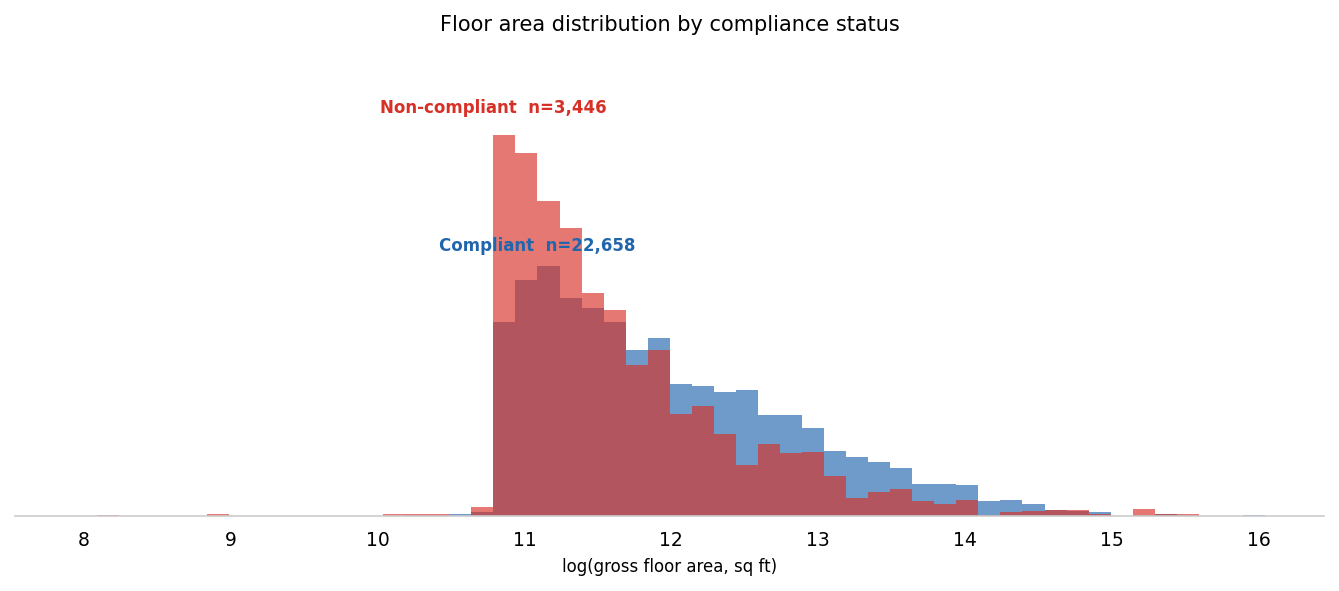
\includegraphics[width=0.72\linewidth]{figures/fig_05_floor_area_by_compliance.png}
\caption*{\textbf{Figure 4.2. Floor area distribution for compliant and non-compliant buildings.} Restricted to the 26,104 records with an observed floor area (compliant $n = 22{,}658$, non-compliant $n = 3{,}446$); floor area is null for the remainder, disproportionately among non-compliant records. Compliant buildings are systematically larger: the compliant median (131,000 sq ft) is 41\% larger than the non-compliant median (92,966 sq ft), and the two distributions diverge with size, though they overlap. Building size is the clearest correlate of compliance in the data. Author's analysis of Chicago Energy Benchmarking data (\cit{citynd}{City of Chicago, n.d.}).}
\end{figure}

The target variable spans five orders of magnitude (Figure 4.3): minimum 0, median 1,026, maximum 185,162 metric tons CO$_2$e (mean 2,493, std 5,995). The distribution is severely right-skewed (the mean is 2.4 times the median), which reflects the multiplicative relationship between building size and emissions: a building twice as large emits roughly twice as much GHG. On the log$_{1+}$ scale the distribution is approximately Normal. The data record 63 property types, reflecting the heterogeneity of Chicago's building stock; 56 appear among the compliant records, 55 among the subset of those that carry an observed GHG value, which Section 5 uses as the compliant training set (Figure 4.4): multifamily housing dominates (11,278 records), followed by K-12 schools (3,503) and offices (3,214). Prior work on benchmarking prediction uses the observed compliant sample directly, without accounting for the compliance gate that produced it (\cit{hsu2015}{Hsu, 2015}; \cit{kontokostatull2017}{Kontokosta \& Tull, 2017}).

\begin{figure}[tbp]
\centering
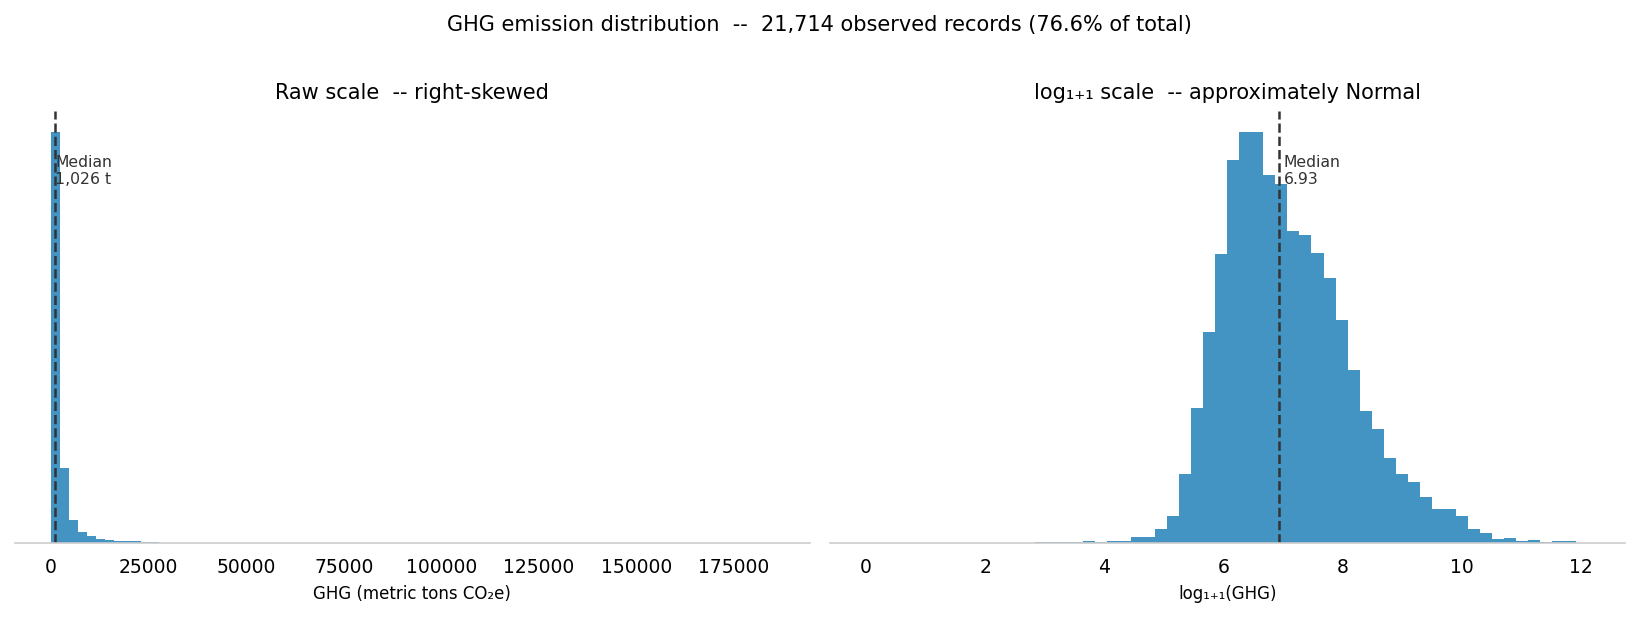
\includegraphics[width=0.86\linewidth]{figures/fig_02_ghg_distribution.png}
\caption*{\textbf{Figure 4.3. GHG emission distribution on raw and log$_{1+}$ scale (observed records only, $n = 21{,}714$).} The raw distribution is severely right-skewed: the mean (2,493 t) is 2.4$\times$ the median (1,026 t), and the largest building emits 180$\times$ the median building. The log$_{1+}$ transformation produces a distribution close to Normal. Author's analysis of Chicago Energy Benchmarking data (\cit{citynd}{City of Chicago, n.d.}).}
\end{figure}

\begin{figure}[tbp]
\centering
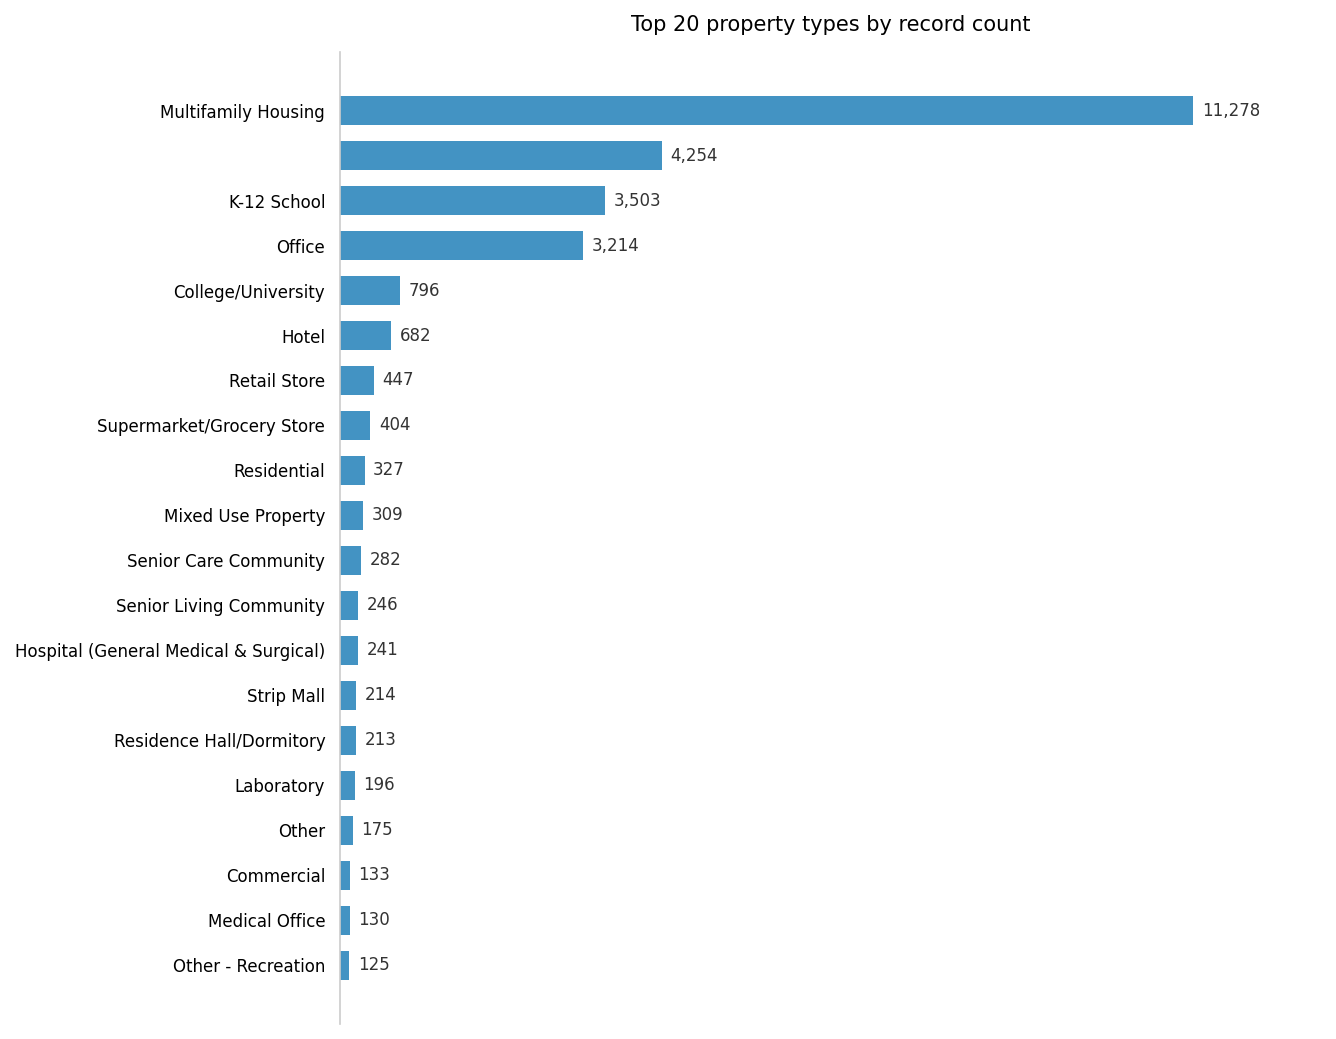
\includegraphics[width=0.58\linewidth]{figures/fig_07_property_type_frequency.png}
\caption*{\textbf{Figure 4.4. Top 20 property types by record count (all 28,329 records).} Multifamily housing accounts for 40\% of all records; the dataset is dominated by residential buildings and public-sector facilities (schools, universities). The bar for missing property type (4,254 records) shows buildings whose type is not recorded in the city registry. Author's analysis of Chicago Energy Benchmarking data (\cit{citynd}{City of Chicago, n.d.}).}
\end{figure}


\subsection{Stage 1 Applied: The Shadow Matrix}

Stage 1 reads the recording layer from the data alone, before any governing document is opened. It needs two things: the compliance indicator $C$ and the structure of co-missingness across the file. The compliance indicator is read, not imputed: $C = 1$ when \code{reporting\_status} is \code{Submitted} or \code{Submitted Data} and the building is not exempt from the Chicago Energy Rating, and $C = 0$ otherwise. The exemption flag is null-filled to false, the conservative reading, since a missing exemption is treated as no exemption. This yields 22,819 compliant records (80.5\%) and 5,510 non-compliant (19.5\%). Because $C$ is observed for every record ($C \in \mathcal{O}$), it can anchor the correlation analysis without itself being subject to missingness.

The obvious first look is the per-variable missing rate (Figure 4.5), and it is the wrong instrument. The most-missing fields are water use (85.7\%) and district steam and chilled water (79.7\%, 79.1\%), yet these are not the gated block. Their blanks are structural: most buildings are not connected to the district energy network, as Section 4.1 noted. The gated outcome and mediator fields sit far lower, clustered near the 23.4\% outcome-missing line: GHG and its intensity (23.4\%), the energy-use intensities (19.3\% to 23.2\%), electricity (18.8\%), and natural gas (24.0\%). A raw rate cannot separate a structural absence from a gate. For that, Stage 1 turns from the rate of missingness to its correlation structure.

\begin{figure}[tbp]
\centering
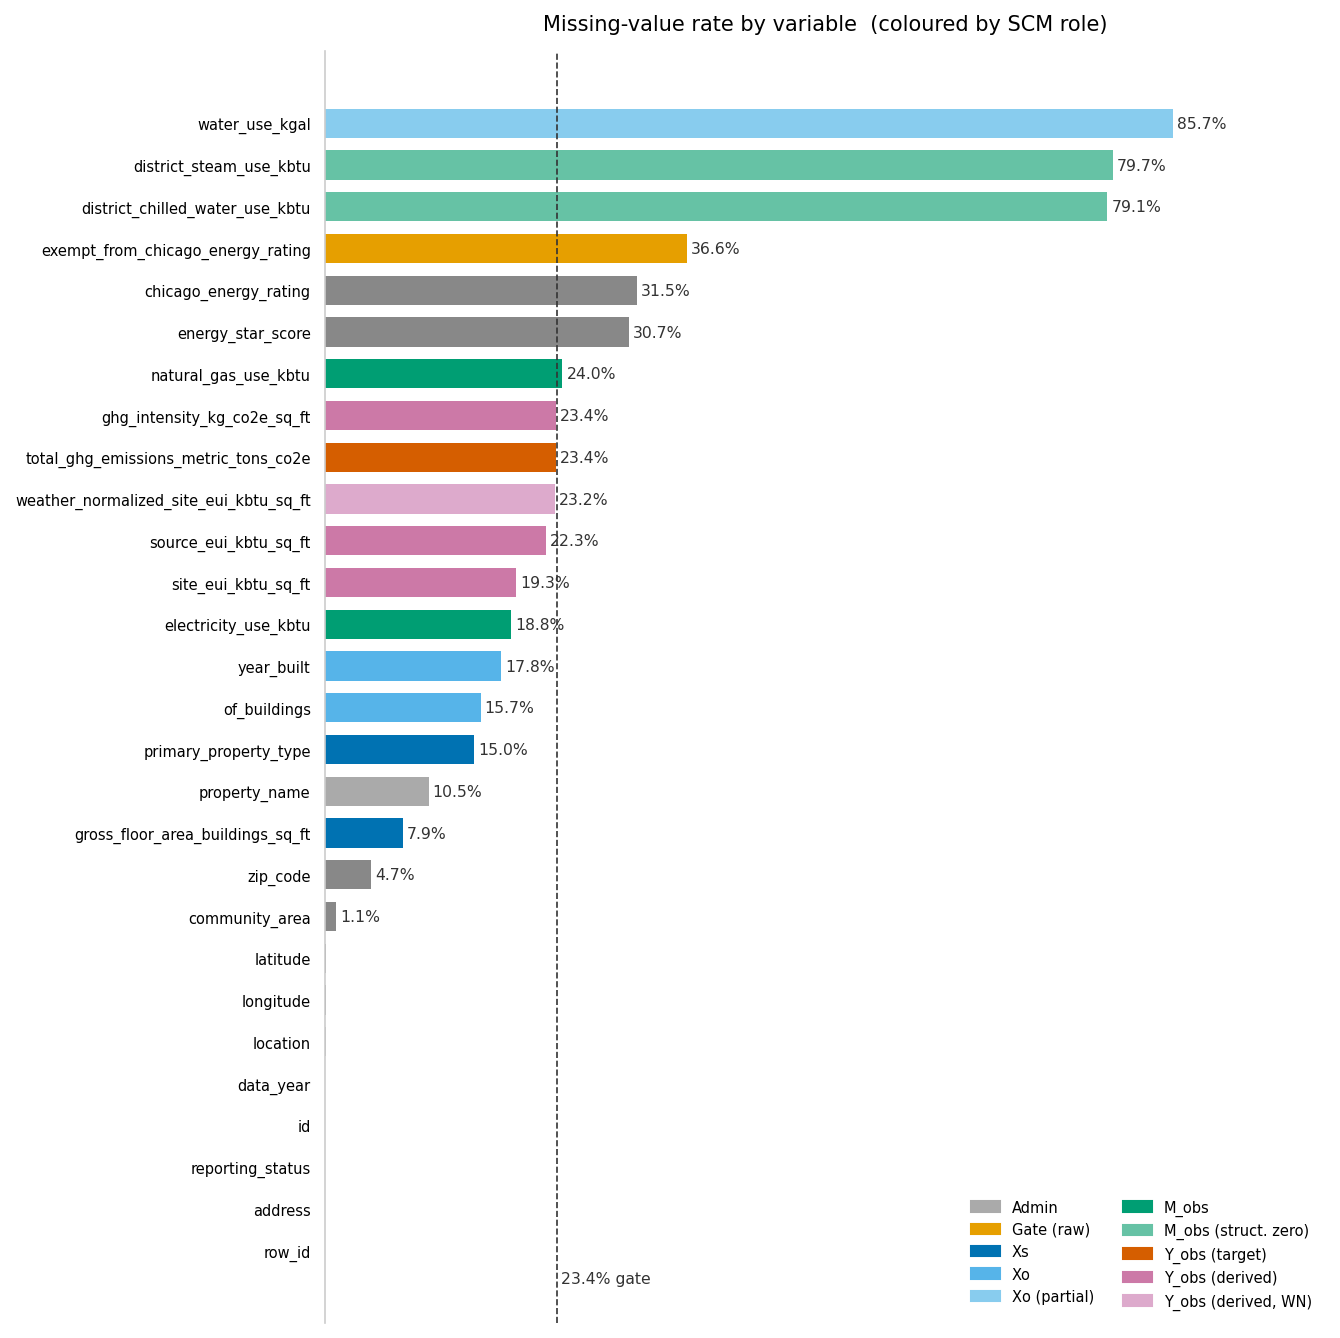
\includegraphics[width=0.80\linewidth]{figures/fig_03_missingness_by_variable.png}
\caption*{\textbf{Figure 4.5. Missing-value rate by variable, coloured by SCM role.} The most-missing fields (water use, district steam and chilled water) are structural absences, not gated fields; the gated mediators and outcomes cluster near the 23.4\% outcome-missing line (dashed). Raw missingness rate does not distinguish a structural zero from a compliance gate. Author's analysis of Chicago Energy Benchmarking data (\cit{citynd}{City of Chicago, n.d.}).}
\end{figure}

The shadow matrix (Figure 4.6) is the matrix of pairwise correlations among the variables' observation indicators, with $C$ appended. The three regimes of Section 3.1 are directly visible. \textbf{Gate alignment:} the gated mediators and derived outcomes correlate strongly with $C$: electricity 0.93, site EUI 0.91, source EUI 0.84, GHG, GHG intensity and weather-normalised EUI 0.83, natural gas 0.80, ENERGY STAR score 0.73. Each field is observed almost exactly when the building complied. \textbf{Block structure:} within that set the observation indicators co-vary between 0.74 and 1.00 (mean 0.88); electricity and site EUI move together at 0.98, and GHG and GHG intensity at 1.00. The fields appear and vanish as a single unit, the fingerprint of an atomic reporting gate (Condition 3 of Definition 2.1). \textbf{Idiosyncratic missingness:} present too, but confined outside the gated block. The geographic coordinates (latitude, longitude, location) correlate near zero with $C$ and with every substantive field ($|r| \approx 0.02$); their blanks carry no information about compliance. The three share a single geocoding source and so co-miss in one small block (15 records, 0.1\%) rather than scattering at random, but the property that matters holds: the shadow matrix sets them cleanly apart from the gate-driven block, which is the discrimination the diagnostic exists to provide.

\begin{figure}[tbp]
\centering
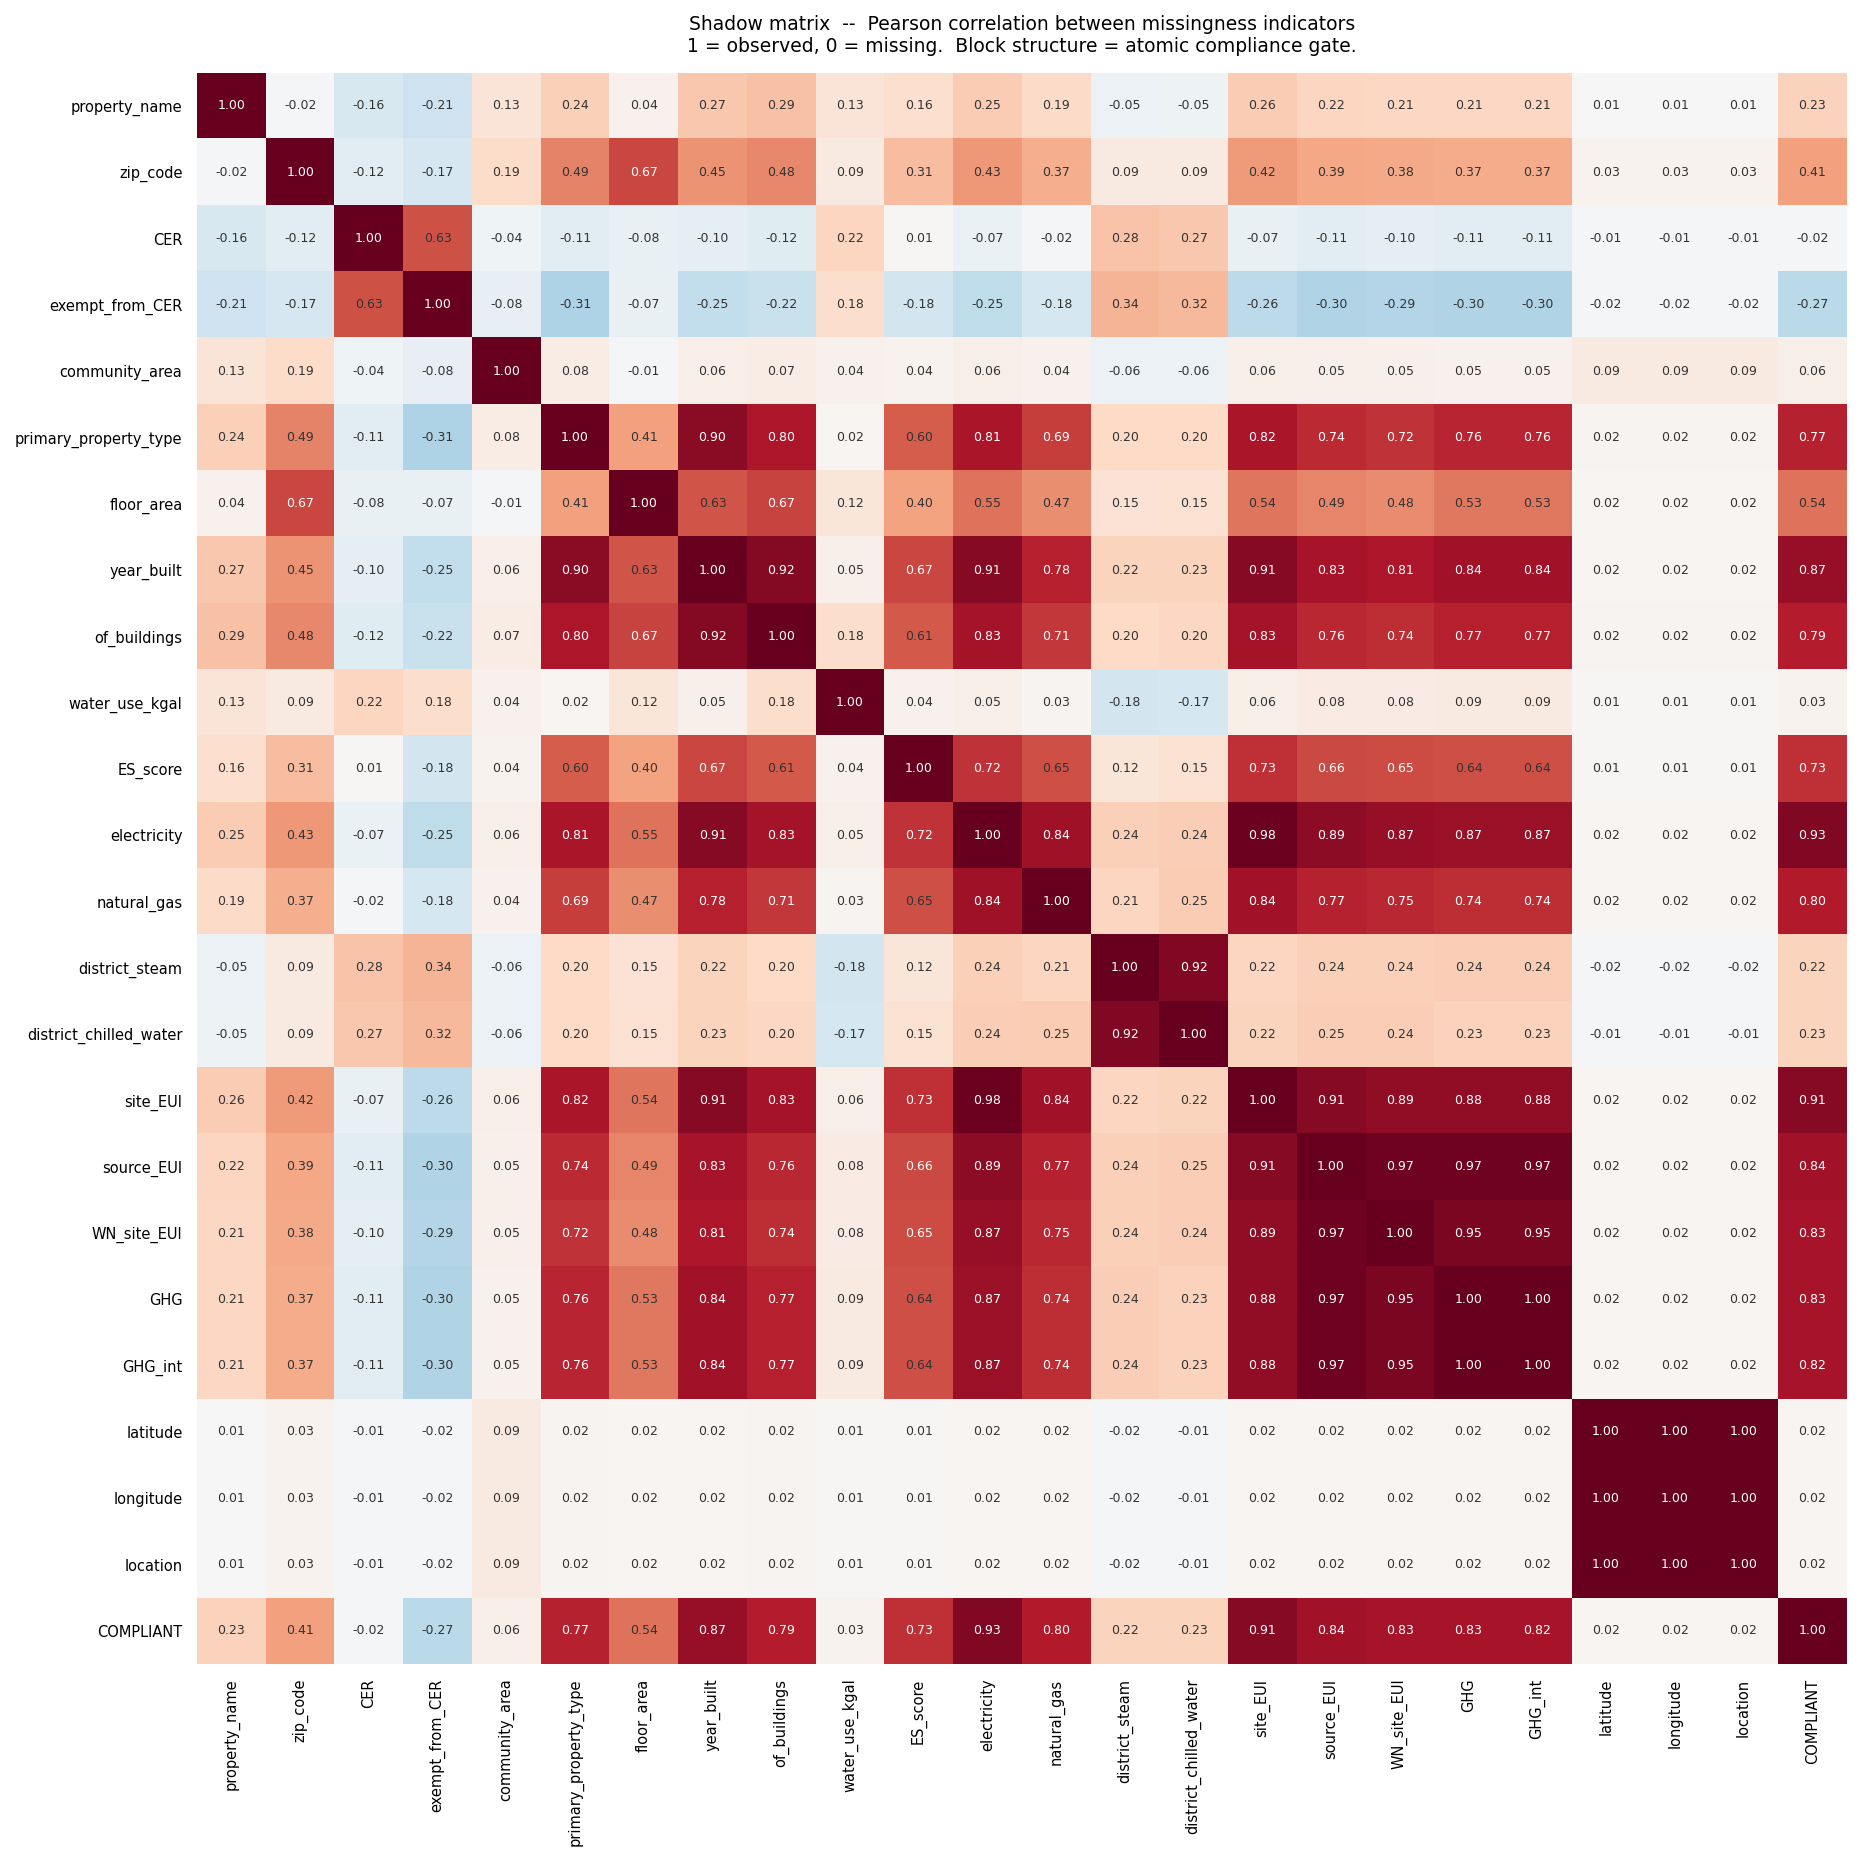
\includegraphics[width=0.80\linewidth]{figures/fig_04_shadow_matrix.png}
\caption*{\textbf{Figure 4.6. Shadow matrix: correlations among observation indicators.} Each cell is the correlation between two fields' missingness, with the compliance indicator appended. The gated mediators and derived outcomes form a dark block that also aligns with compliance; structural zeros, the Chicago Energy Rating, and the upstream and spatial fields sit outside it. Author's analysis of Chicago Energy Benchmarking data (\cit{citynd}{City of Chicago, n.d.}).}
\end{figure}

Three groups sit apart from the gated block, exactly as Section 3.1 anticipates, and reading them out is as much of Stage 1 as identifying the block itself. \textbf{Structural zeros:} district steam and chilled water correlate only 0.22 and 0.23 with $C$. Their blanks track the building's physical configuration, not the gate, and must be preserved as genuine zeros rather than recoded as gated missing. \textbf{The Chicago Energy Rating anomaly:} the rating correlates $-0.02$ with $C$, effectively not at all. Its missingness is governed by the programme's 2018 introduction date rather than compliance, so despite being a performance field it does not belong to the gated block. \textbf{Upstream fields:} floor area, property type, year built and number of buildings correlate with $C$ only moderately and unevenly (0.54 to 0.87); their missingness reflects registry completeness, a separate mechanism Section 4.1 already flagged, so Stage 1 leaves them outside the gated block. Among the spatial fields, only the ZIP code carries a compliance signal (0.41, tracking building size rather than compliance directly); community area and the coordinates carry essentially none.

The block-and-gate pattern is incompatible with data missing completely at random, under which every off-diagonal correlation would be zero (\cit{littlerubin2002}{Little \& Rubin, 2002}). Refuting that hypothesis rules out the default workflows, complete-case analysis and unconditional imputation, and forces the structural treatment that follows. Stage 1's output is a map of the observation structure, established from the data alone and independently of the documents Stage 3 will test against: the gate $C$; the gated block $\{M^{\text{obs}}, Y^{\text{obs}}\}$ of energy mediators and derived performance fields; the structural zeros to be preserved; and the upstream and spatial fields, whose lighter missingness is registry- or geocoding-driven and unrelated to the gate. The map stops at this partition. It shows the gated fields moving as one block but cannot, from co-missingness alone, separate the outcome within that block from the mediators that produce it. That separation is the work of Stage 2.


\subsection{Stage 2 Applied: The Candidate DAG}

Stage 2 turns the Stage 1 map into a candidate causal graph of the world layer that generated the Chicago data. The materials are deliberately limited to the shadow matrix, the variable descriptions, and Definition 2.1; the benchmarking ordinance and the EPA accounting standard stay closed until Stage 3, so the graph and the documents that will test it remain independent. The five-step procedure of Section 3.2 applies directly; Figure 4.7 shows the candidate DAG it produces.

\begin{figure}[H]
\centering
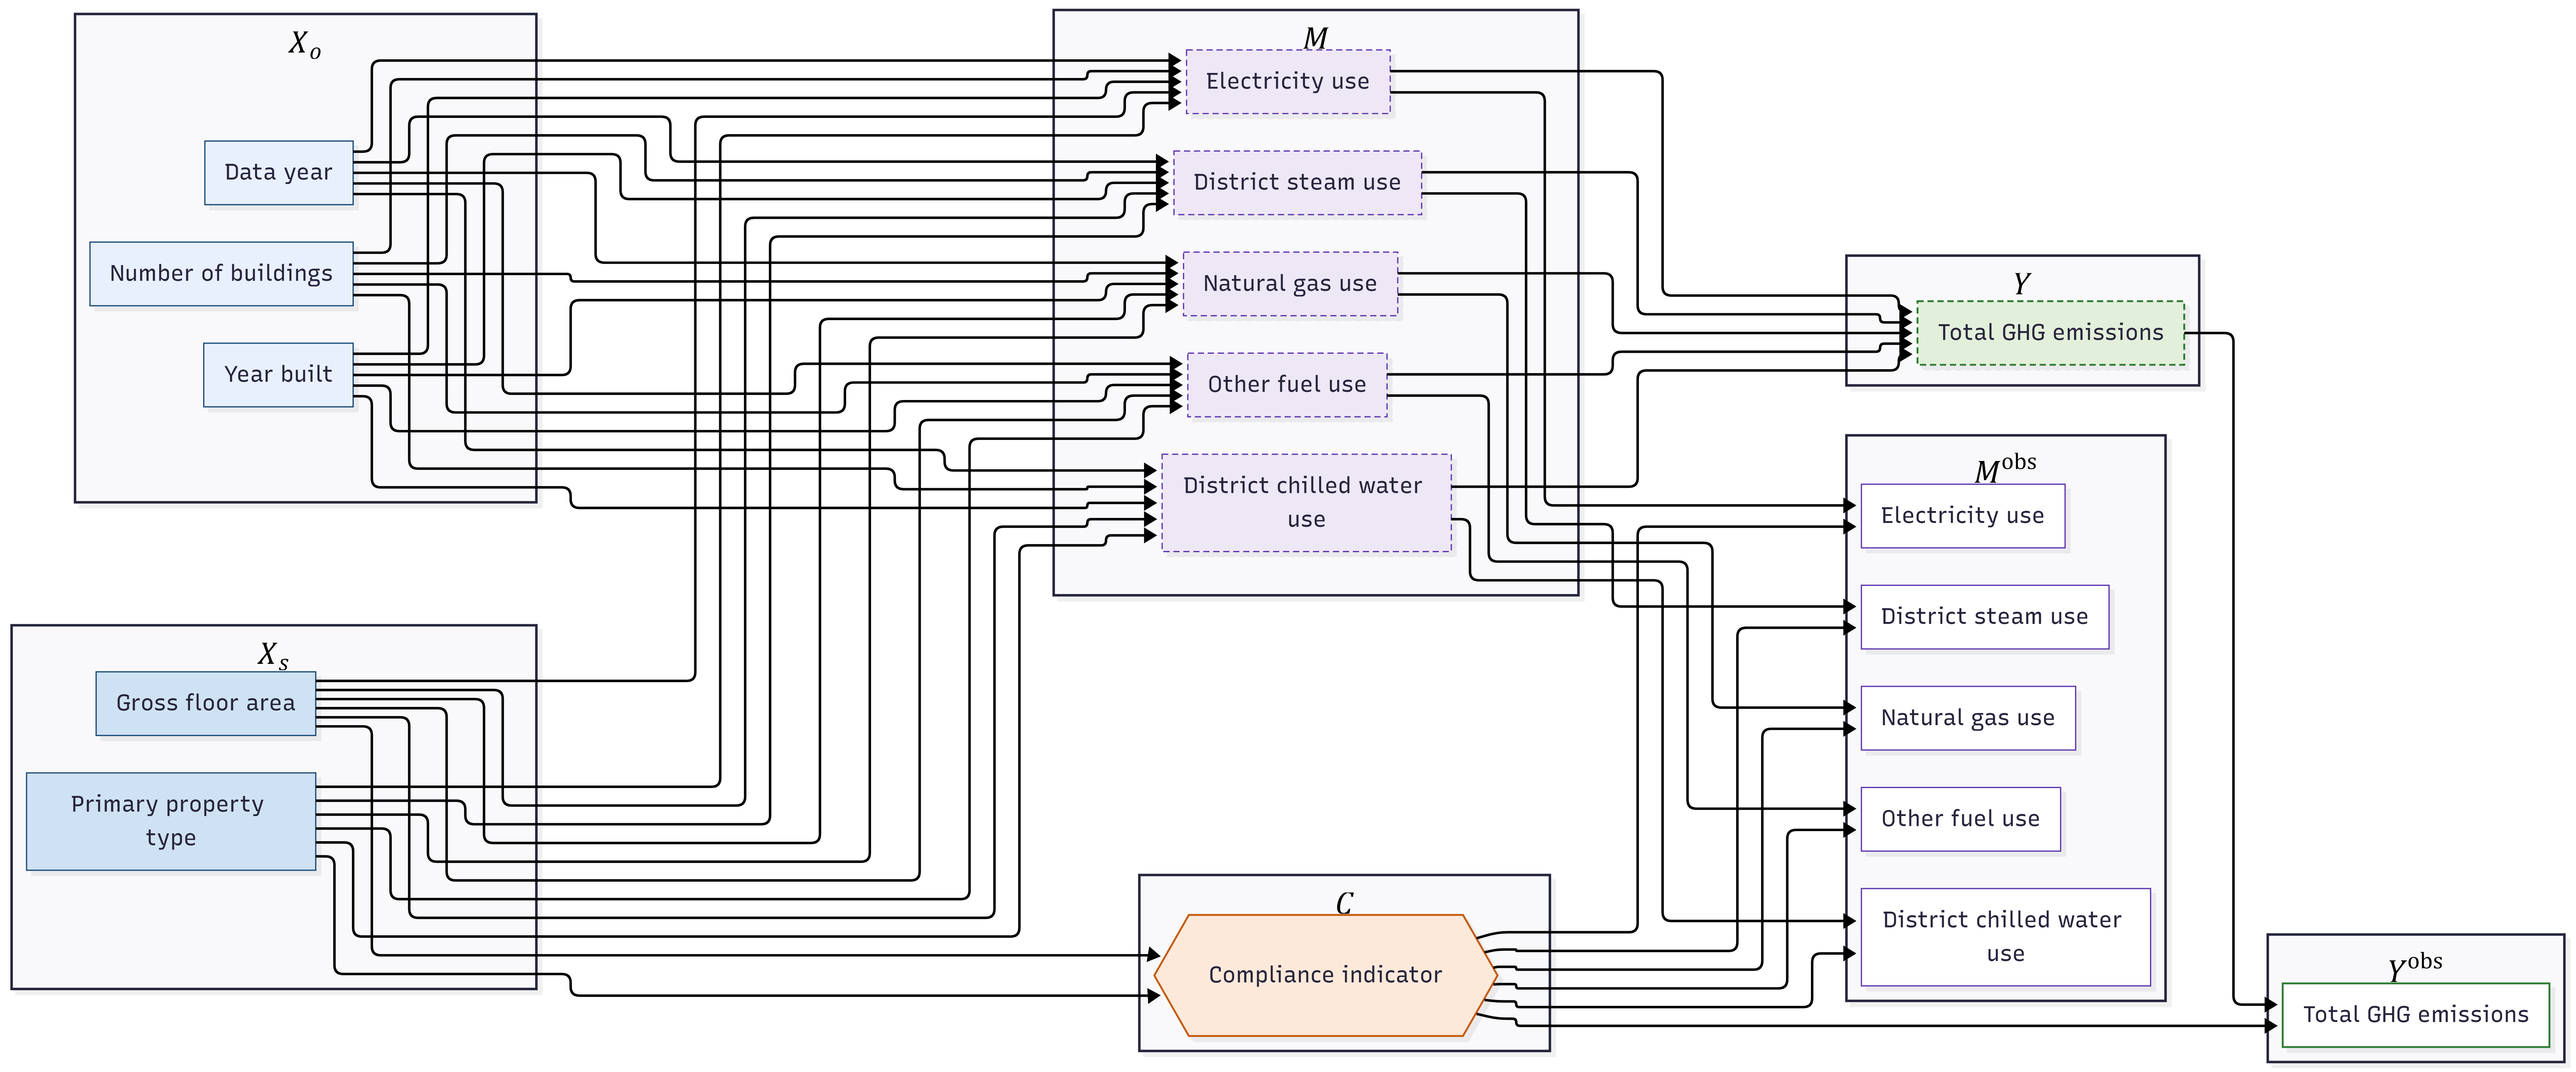
\includegraphics[width=0.98\linewidth]{figures/figure4_7.png}
\caption*{\textbf{Figure 4.7. Candidate DAG for the Chicago data (Stage 2 output).} The Definition 2.1 template instantiated with the Chicago variables, one node per variable. The selection variables $\mathbf{X}_s$ (gross floor area, primary property type) cause the compliance gate $C$ and, with the non-selection features $X_o$ (year built, number of buildings, data year), the latent energy mediators $M$ (electricity, natural gas, district steam, district chilled water, other fuel use); the mediators produce the latent outcome $Y$ (total GHG emissions). The gate $C$ governs the recorded layers $M^{\text{obs}}$ and $Y^{\text{obs}}$: each recorded field equals its latent value when $C = 1$ and is missing otherwise (the colliders $M \to M^{\text{obs}} \leftarrow C$ and $Y \to Y^{\text{obs}} \leftarrow C$). Latent nodes are dashed. Author's construction from the shadow matrix, variable descriptions, and Definition 2.1.}
\end{figure}

\textbf{Step 1. Carry over the partition (data).} From Stage 1: the gate $C$ is fixed; the gated block $\{M^{\text{obs}}, Y^{\text{obs}}\}$ holds the metered energy fields and the derived performance fields that co-miss with $C$; the structural zeros (district steam, district chilled water) are flagged as physical absences to preserve; and the upstream set holds the building characteristics, whose lighter missingness is unrelated to the gate. The shadow matrix shows the gated block as one undifferentiated group: it cannot, on its own, tell the outcome within it from its mediators (Section 4.2).

\textbf{Step 2. Name the outcome $Y$ (choice).} The research question fixes $Y$ as total GHG emissions (\code{total\_ghg\_emissions\_metric\_tons\_co2e}), the quantity the programme exists to measure. The other gated performance fields (the energy-use intensities, GHG intensity, and ENERGY STAR score) are further performance measures derived from the same mediators rather than the target; the graph admits them as a fan of co-outcomes (Section 3.2), but the study tracks total GHG.

\textbf{Step 3. Reason the mediators $M$ (conjecture).} Among the remaining gated fields, five metered energy quantities (electricity, natural gas, district steam, district chilled water, and other fuel use) are, by the descriptions, the channels through which a building's characteristics produce emissions. They are taken as the mediators $M$ feeding $Y$, giving the structural claim $\mathrm{pa}(Y) = M$. District steam and chilled water enter $M$ as structural zeros for buildings off the district network (Section 4.1). This separation of mediators from outcome is made by argument; the shadow matrix cannot perform it.

\textbf{Step 4. Reason the selection variables $\mathbf{X}_s$ (conjecture).} Within the upstream set, gross floor area is the feature the descriptions mark as a measure of building size, the kind of eligibility criterion a threshold gates on (Condition 1), and primary property type is a categorical eligibility criterion of the same kind. They are taken as $\mathbf{X}_s$; year built and number of buildings are $X_o$, upstream causes of energy use that play no part in selection, alongside the data year, a yearly fixed effect that captures annual variation in energy consumption (weather, prices, code changes) rather than a building characteristic. The data corroborate the floor-area conjecture: compliant buildings are scarce at small sizes and predominate as size grows (Figure 4.2), consistent with floor area as the selection variable. Realized compliance is not perfectly sharp, so the signature is suggestive, not decisive, and speaks only to selection; whether the documented rule actually reads floor area and property type is reserved for Stage 3.

\textbf{Step 5. Instantiate the edges (template).} With the roles assigned, Definition 2.1 supplies every edge with no further argument: $\mathbf{X}_s \to C$, $\mathbf{X}_s \to M$ and $X_o \to M$, $M \to Y$, and the institution layer $M \to M^{\text{obs}} \leftarrow C$ with $Y \to Y^{\text{obs}} \leftarrow C$. The result is Figure 2.1's template with each role expanded into its Chicago variables (Figure 4.7).

The candidate DAG makes three predictions that Stage 3 will set against the documents:

\begin{enumerate}
  \item \textbf{P1 (selection):} compliance is caused by the upstream characteristics $\mathbf{X}_s$, not by energy use or emissions; the gate reads building size and type, nothing downstream.
  \item \textbf{P2 (atomic gate):} the mediators and the outcome are observed or withheld as a single unit governed by $C$, a prediction the shadow-matrix block of Section 4.2 already corroborates in the data.
  \item \textbf{P3 (mediator sufficiency):} $\mathrm{pa}(Y) = M$, so total emissions are a function of the metered energy mediators alone, with no direct parent outside $M$.
\end{enumerate}

P3 is the sharpest and least supported claim. Nothing in the shadow matrix, which cannot separate the outcome from its mediators inside the gated block, can establish it; it rests for now on the variable descriptions alone. Stage 3 tests it against the EPA accounting standard that fixes how emissions are computed from metered energy, and tests the selection and classification claims against the ordinance (Section 4.4).


\subsection{Stage 3 Applied: Falsification and Conformance}

Stage 3 tests the candidate DAG against documents that took no part in building it, so any clash would be genuine evidence against the graph rather than circular confirmation. The graph came from the shadow matrix, the variable descriptions, and Definition 2.1 alone (Section 4.3), while the benchmarking ordinance, the reporting schema, and the EPA accounting standard were held back for exactly this purpose. Set against the three predictions that close Section 4.3, none of these documents contradicts the graph.

The ordinance defines a building's duty to report by its size and property class, settling the selection prediction. Under the Municipal Code of Chicago, Chapter 18-14 (\cit{city2013}{City of Chicago, 2013}), a building is ``covered'' on two upstream characteristics only, a gross floor area at or above 50,000 square feet and a property class, with municipal, commercial, and residential buildings drawn in and named categories (stadiums, industrial and manufacturing facilities, storage and hazardous-material buildings) exempted. Covered owners must benchmark in ENERGY STAR Portfolio Manager and file each year. Floor area and property type are exactly the two variables Step 4 assigned to $\mathbf{X}_s$, and the duty turns on no energy or emissions quantity, which a building has not reported when its obligation is set. The phased rollout corroborates the same edge from a second direction: eligibility was extended by size and class over three cycles (commercial above 250,000 sq ft in 2014; commercial 50,000 to 250,000 and residential above 250,000 in 2015; residential 50,000 to 250,000 in 2016), and the record counts climb in step (Figure 4.1). Because the thresholds were switched on year by year, the same rollout also gives the data year a transient role in the gate, which the refinement below makes explicit.

A single annual Portfolio Manager submission carries every metered and derived field at once, so the atomic gate needs no separate document: the one-report obligation makes the whole block appear or vanish together. The shadow matrix already showed exactly this pattern in Stage 1 (Section 4.2).

The mediator/outcome split is the reporting schema's own, not the DAG's invention: a building enters site energy per fuel (electricity, natural gas, district steam, district chilled water, and minor others), and Portfolio Manager derives Total GHG Emissions, site and source EUI, and the ENERGY STAR score from those meters (\cit{epa2025}{U.S. EPA, 2025}). The five metered quantities are therefore $M$, total GHG is $Y$, and the remaining performance fields are the co-outcome fan, each a further function of the same meters rather than a parent of $Y$.

The accounting standard then makes the sufficiency claim itself explicit, computing emissions by ``multiplying the site energy for each fuel by the emissions factor for that specific fuel type'' and summing across fuels (\cit{epa2025}{U.S. EPA, 2025}), which is exactly the additive form $\mathrm{pa}(Y) = M$ requires:

\[
\mathrm{GHG} = \sum_{f} \phi_f\, E_f .
\]

Here $E_f$ is the site energy the building draws from fuel $f$ and $\phi_f$ is that fuel's emission factor, the sum running over the metered fuels. The standard fixes each $\phi_f$ as a published constant, a national value for each combustion and district fuel and a regional, year-specific eGRID factor for electricity (Table 4.2).

Because every $\phi_f$ is set outside the building, the standard makes $Y$ a deterministic function of the metered fuels, which is P3 in the institution's own terms: among building characteristics, none parents $Y$ except through the meters. Whether the recorded data actually obey the formula is a separate, quantitative question, taken up below.

The documentary comparison settles the structure; two data-side checks corroborate it where the data can speak: an outcome reconstruction (does $M$ recover $Y$?) and an upstream-to-mediator regression (does $X$ drive $M$?), both drawn from the full panel of 28,329 building-year records (2014--2023) and prepared as follows.

\begin{enumerate}
  \item \textbf{Reconstruction.} The 21,704 records with an observed GHG value and finite, non-negative energy (the energy filter removes 10 of the 21,714 GHG-observed records of Table 4.1); the regressors are the four metered fuels (electricity, gas, district steam, district chilled water), each unreported or off-network value set to zero, with other fuel (observed for 0.3\% of records) negligible and excluded.
  \item \textbf{Upstream regression.} Per mediator, the records with that mediator observed and all five upstream features present (floor area $> 0$).
  \item \textbf{Transforms.} The reconstruction is linear, since the documented accounting is additive; the upstream regression takes $\log(1+M)$ on $\log(\text{floor area})$ (so the coefficient is an elasticity), with year built and number of buildings entering linearly and property type and data year as fixed effects.
\end{enumerate}

Mediators are recorded only for the (largely) compliant units, so both fits sit on that subsample; conditioning on the upstream features that drive selection keeps $E[M \mid X]$ unbiased there.

Because the checks ask whether a connection exists and conforms, not what a coefficient is to three decimals, the tables report $R^2$ (decomposed by block), the full-model adjusted $R^2$ (to confirm the fit is not inflated by the parameter count), the floor-area elasticity, and the recovered emission factors. Standard errors and test statistics are omitted, since with $n$ in the tens of thousands they would be uniformly significant and would over-weight a check subordinate to the documentary test.

If $\mathrm{pa}(Y) = M$ and the recorded outcome implements the documented formula, total emissions must reconstruct as a near-exact linear combination of the metered fuels, so the first check fits that same identity to the records, now with a residual to absorb any departure:

\[
\mathrm{GHG}_i = \sum_{f \in \mathcal{F}} \phi_f\, E_{if} + \varepsilon_i ,
\qquad \mathcal{F} = \{\text{electricity, gas, steam, chilled water}\}.
\]

Here $\mathrm{GHG}_i$ and $E_{if}$ are the emissions and the fuel-$f$ energy recorded for building-year $i$, $\phi_f$ is the fitted factor for fuel $f$, $\mathcal{F}$ is the set of metered fuels, and $\varepsilon_i$ is the residual.

Because the electricity grid decarbonises year on year, we also fit a variant in which electricity carries a year-specific factor while the combustion fuels stay constant:

\[
\mathrm{GHG}_i = \sum_{t} \phi^{\text{elec}}_{t}\, \mathbf{1}\{\text{year}_i = t\}\, E_{i,\text{elec}} + \sum_{f \neq \text{elec}} \phi_f\, E_{if} + \varepsilon_i .
\]

Here $\phi^{\text{elec}}_t$ is a separate electricity factor for each data year $t$, $\mathbf{1}\{\text{year}_i = t\}$ selects the year of record $i$, and the combustion and district fuels keep the single factor $\phi_f$ of the first variant.

\par\medskip\noindent
{\small\itshape \textbf{Table 4.2. Recovered emission factors against the EPA standard.} For each metered fuel: the EPA-prescribed emission factor (\cit{epa2025}{U.S. EPA, 2025}) and the factor recovered by the no-intercept reconstruction above ($n = 21{,}704$). $^\ddagger$Electricity has no single EPA value, taking a year-specific regional eGRID factor (Chicago's RFCW subregion, 121.78 in 2023, higher earlier); the recovered 169.1 is the multi-year average (see text). Author's analysis of Chicago Energy Benchmarking data (\cit{citynd}{City of Chicago, n.d.}).\par}
\nopagebreak\medskip\nopagebreak
{
\setlength{\tabcolsep}{7pt}
\renewcommand{\arraystretch}{1.15}
\begin{longtable}{lrr}
\toprule
Fuel & EPA factor (kg CO$_2$e/MBtu) & Recovered factor \\
\midrule
\endfirsthead
\toprule
Fuel & EPA factor (kg CO$_2$e/MBtu) & Recovered factor \\
\midrule
\endhead
\bottomrule
\endlastfoot
Electricity & eGRID RFCW, annual$^\ddagger$ & 169.1 \\
Natural gas & 53.11 & 53.7 \\
District steam & 66.40 & 58.2 \\
District chilled water & 49.31--73.89 & 49.3 \\
\end{longtable}
}
\par\medskip

The reconstruction confirms that the recorded emissions follow the documented formula, in three respects.

\begin{enumerate}
  \item \textbf{$\mathrm{pa}(Y) = M$.} A constant factor per fuel reproduces almost all of emissions ($R^2 = 0.987$), and a year-specific electricity factor makes the fit essentially exact ($0.9999$, the adjusted $R^2$ identical at this $n$), with no role for a parent of $Y$ outside $M$.
  \item \textbf{The residual is a documented trend, not noise.} The $0.987 \to 0.9999$ gain is entirely electricity's factor falling year on year (201 to 132 kg CO$_2$e/MBtu over 2014--2022), the grid decarbonising toward the published 2023 RFCW value: the auditable disturbance $U_Y$ with a diagnosable cause.
  \item \textbf{The factors conform to the standard.} Natural gas matches almost exactly (53.7 against the EPA-prescribed 53.11), and district chilled water lands on the engine-driven-chiller value (49.3 against 49.31). District steam runs below the documented value (58.2 against 66.40), the few buildings on the district network leaving its coefficient noisy. Electricity has no single benchmark: its recovered 169.1 is the multi-year average of a factor declining year on year (Table 4.2 note).
\end{enumerate}

Selection bias exists only if the upstream features drive the mediators (Condition 2), so the second check must establish that edge from the data. Because the mediators are metered rather than computed, no document speaks to the edge; it can be corroborated only by association: we regress each mediator on the upstream features,

\[
\log(1 + M_{if}) = \beta_0 + \beta_A\, \log A_i + \sum_p \gamma_p\, \mathbf{1}\{\text{type}_i = p\} + \sum_t \delta_t\, \mathbf{1}\{\text{year}_i = t\} + \theta_1\, \text{built}_i + \theta_2\, \text{nbldg}_i + \varepsilon_{if} ,
\]

Here $M_{if}$ is the fuel-$f$ energy and $A_i$ the gross floor area of building-year $i$; the indicators $\mathbf{1}\{\cdot\}$ encode property type $p$ and data year $t$; $\text{built}_i$ and $\text{nbldg}_i$ are the year built and number of buildings; $\beta_A$ is the floor-area elasticity, reported from the full model, and $\beta_0, \gamma_p, \delta_t, \theta_1, \theta_2$ are the remaining coefficients, with residual $\varepsilon_{if}$.

We fit it in nested blocks (floor area; $+$ property type; $+$ the rest), recording $R^2$ after each, so the column-to-column gains in Table 4.3 give each block's contribution.

\par\medskip\noindent
{\small\itshape \textbf{Table 4.3. Upstream features as drivers of the mediators.} Nested OLS of $\log(1+M)$ adding one block at a time: floor area [$R^2$ (area)], $+$ property type [$R^2$ (+ type)], $+$ year built, number of buildings, and data year [$R^2$ (full)]; the column-to-column gains give each block's contribution, and $\beta_A$ is the floor-area elasticity from the full model. Adjusted $R^2$ (full) differs from $R^2$ (full) by at most 0.001, so the fit is not inflated by the parameter count. The last row totals the metered fuels. Author's analysis of Chicago Energy Benchmarking data (\cit{citynd}{City of Chicago, n.d.}).\par}
\nopagebreak\medskip\nopagebreak
{
\footnotesize
\setlength{\tabcolsep}{5pt}
\renewcommand{\arraystretch}{1.15}
\begin{longtable}{lrrrrrr}
\toprule
Mediator & $n$ & $R^2$ (area) & $R^2$ (+ type) & $R^2$ (full) & adj. $R^2$ (full) & $\beta_A$ \\
\midrule
\endfirsthead
\toprule
Mediator & $n$ & $R^2$ (area) & $R^2$ (+ type) & $R^2$ (full) & adj. $R^2$ (full) & $\beta_A$ \\
\midrule
\endhead
\bottomrule
\endlastfoot
Electricity & 22,724 & 0.467 & 0.544 & 0.567 & 0.567 & 1.03 \\
Natural gas & 21,253 & 0.045 & 0.123 & 0.183 & 0.182 & 0.76 \\
District steam & 5,677 & 0.000 & 0.408 & 0.811 & 0.810 & 0.03 \\
District chilled water & 5,837 & 0.092 & 0.224 & 0.769 & 0.768 & 0.46 \\
Total metered energy & 22,723 & 0.438 & 0.472 & 0.488 & 0.487 & 0.94 \\
\end{longtable}
}
\par\medskip

The regression shows that the upstream features do drive the mediators, in two patterns.

\begin{enumerate}
  \item \textbf{Size drives the dominant mediators.} For electricity and total energy $\beta_A \approx 1$ (doubling floor area roughly doubles energy), with floor area alone explaining 44--47\%, so $\mathbf{X}_s$ is genuinely among the causes of $M$ and the bias is real; $\beta_A \approx 1$ also confirms floor area and energy are on consistent units.
  \item \textbf{The others load on type, not size.} For natural gas and the district fuels, floor area alone explains little (each with $R^2$ (area) below 0.10); property type lifts natural gas from $0.05$ to $0.12$ and carries the district fuels (steam $0.00 \to 0.41$). Gas is system-dependent, and the district fuels are structural zeros whose presence tracks type and location.
\end{enumerate}

The two checks corroborate the structure without carrying its weight, for two reasons. First, a regression reveals association, not direction. Orientation comes from outside the data: $M \to Y$ from the documented formula, which computes emissions from energy, and $X \to M$ from physical and temporal order, since building characteristics precede and produce energy use. Second, neither check is load-bearing for the selection correction's validity, which rests on the documented gate and $\mathrm{pa}(Y) = M$; together they establish only that the connections exist and conform to the documented accounting.

The tests refine the graph as well as confirm it, but the core survives intact: $\mathrm{pa}(Y) = M$ holds to $R^2 = 0.9999$, no mediator is missing, and no building feature parents $Y$ except through the meters.

The refinement falls in one place, the data year, which Figure 4.7 filed among the non-selection features $X_o$ on the hypothesis that it was an ordinary upstream characteristic. Stage 3 overturns that: the data year is the panel's period index rather than a building feature, so the refined DAG lifts it out of the partition (Figure 4.8), where it gains two edges the $X_o$ reading had missed, while year built and number of buildings keep their single edge to $M$:

\begin{enumerate}
  \item \textbf{Data year to $Y$.} Beyond driving energy use (its $\to M$ edge), the data year also acts on the energy-to-emissions conversion: the reconstruction's residual is the eGRID electricity factor falling year on year (inference 2 above), a documented and exogenous influence on $Y$ that Figure 4.7 had absorbed into the disturbance $U_Y$.
  \item \textbf{Data year to $C$.} The phased rollout makes eligibility itself time-varying through 2017, as the threshold fell from 250,000 to 50,000 square feet by class, so the data year enters the gate during the phase-in and the candidate reading that kept it out of selection (Step 4) is corrected.
\end{enumerate}

A further change is to functional form rather than topology: the ordinance fixes $\mathbf{X}_s \to C$ as a sharp threshold at 50,000 square feet with a property-class exemption, not the smooth dependence the candidate edge left implicit.

None of this costs the analysis anything. The data year is observed for every record (Table 4.1) and is already conditioned on in both the propensity and outcome models, so the backdoor the new edges open, $C \leftarrow \text{data year} \rightarrow Y$, is already blocked; the edges only reclassify parts of $U_C$ and $U_Y$ as documented, observed causes. Figure 4.8 records the result.

\begin{figure}[H]
\centering
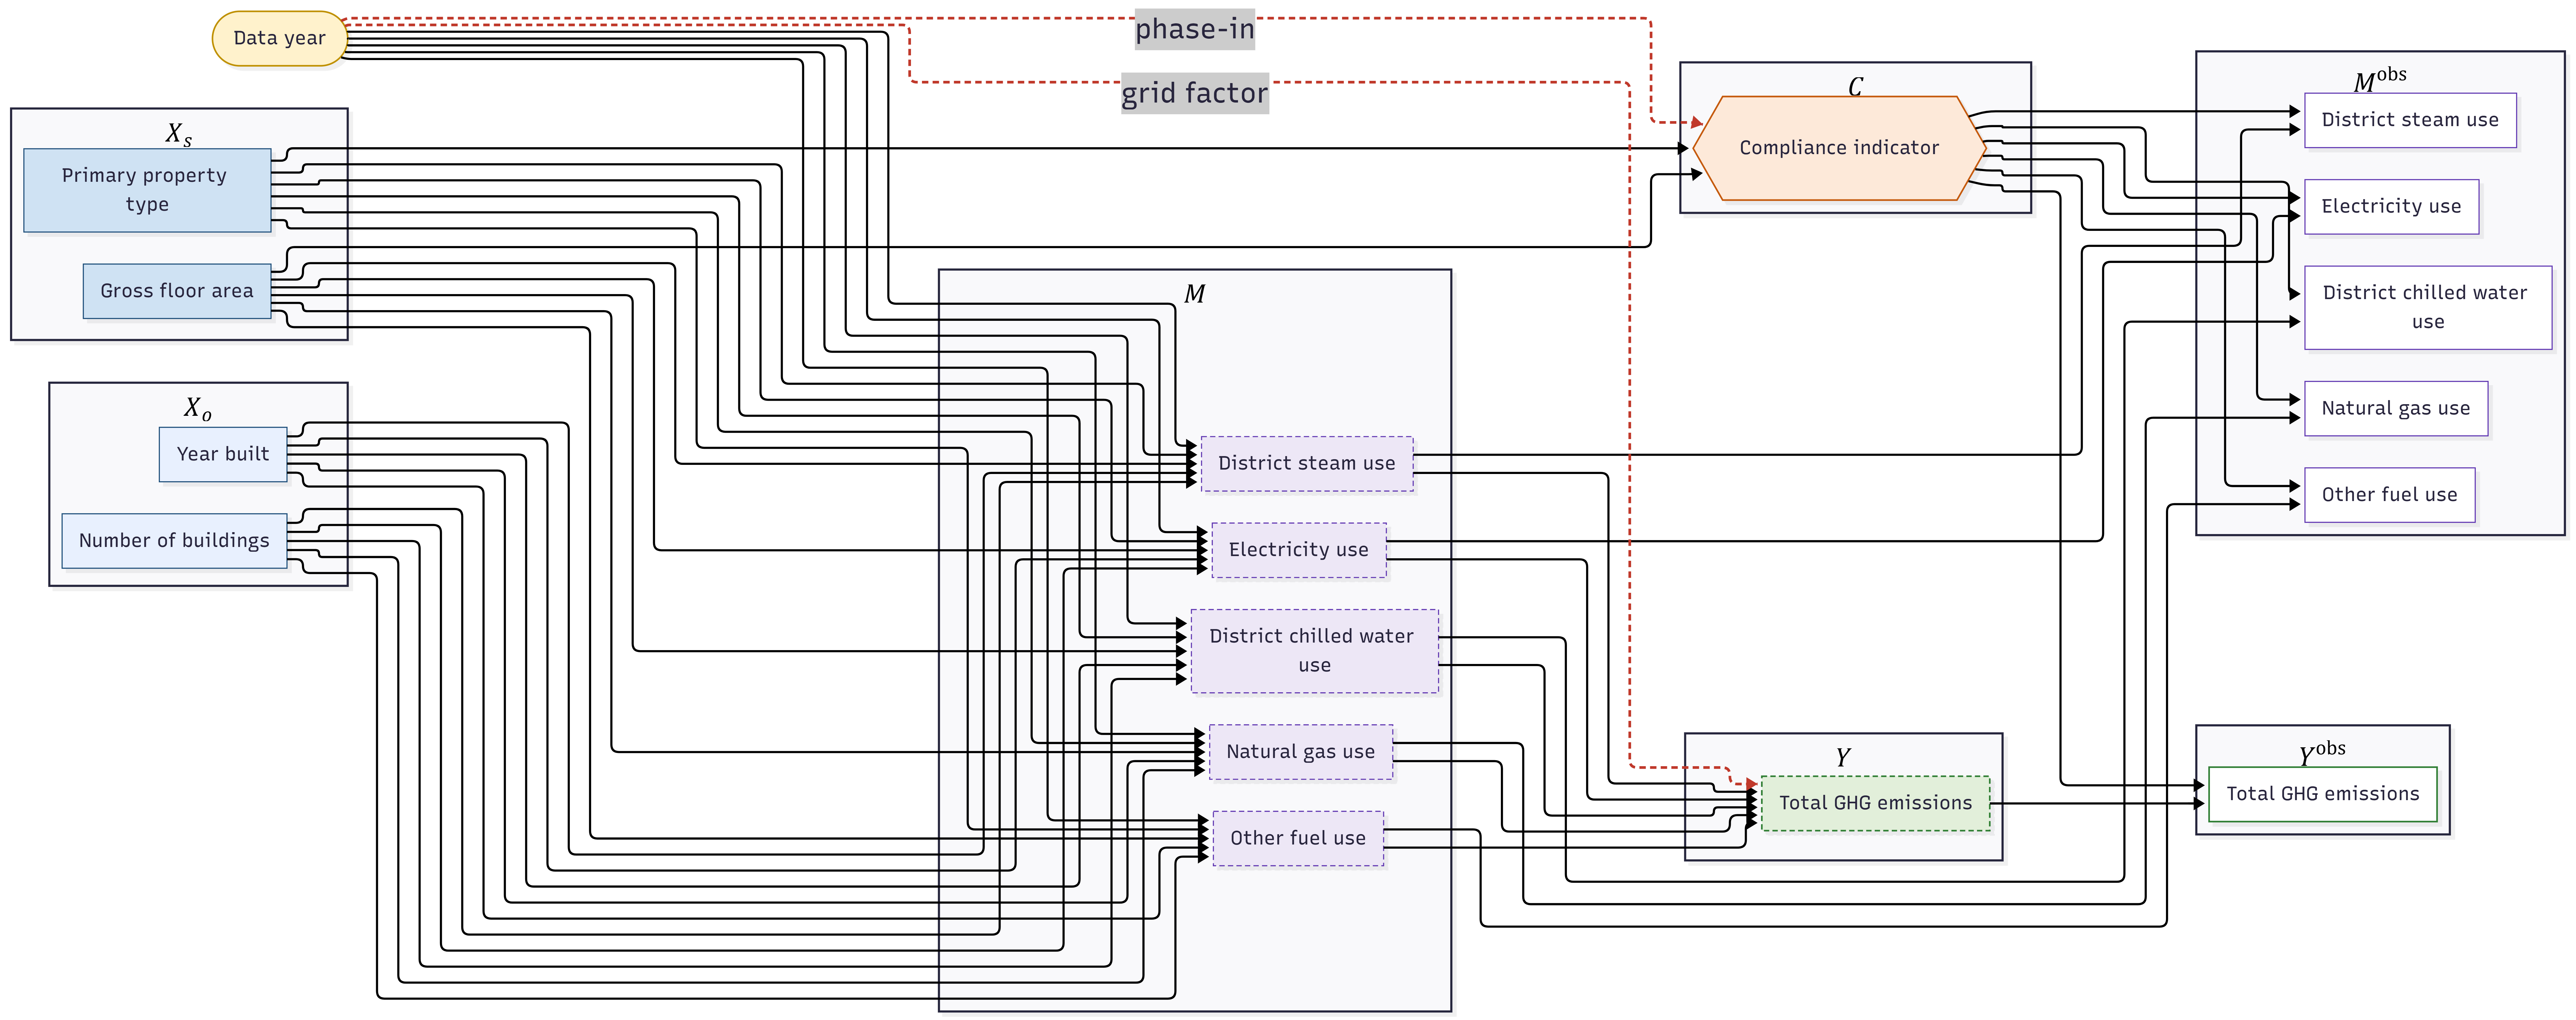
\includegraphics[width=0.98\linewidth]{figures/figure4_8.png}
\caption*{\textbf{Figure 4.8. Tested DAG for the Chicago data (Stage 3 output).} The candidate DAG of Figure 4.7 with the Stage-3 correction: the data year is lifted out of $X_o$ into a standalone period index and gains two edges (highlighted), one to the outcome $Y$ and one to the gate $C$ (see text). All other edges carry over from Figure 4.7; latent nodes are dashed-bordered. Author's construction.}
\end{figure}

All three predictions survive contact with documents that took no part in drawing the graph, and the two regressions add quantitative corroboration where the data can speak. The graph that results is a tested object rather than an asserted one (Figure 4.8): its selection edge is the ordinance's eligibility rule, its mediator/outcome split is the reporting schema's input/output distinction, and its $\mathrm{pa}(Y) = M$ claim is the EPA accounting identity, recovered from the data to $R^2 = 0.9999$. That is the warrant Sections 5 to 7 draw on when they run the full Pearlian analysis on the tested structure.

